\documentclass{article}[12pt]

\usepackage{graphicx}
\usepackage{footnote}
\usepackage{multirow}
\makesavenoteenv{tabular}
\makesavenoteenv{table}

\begin{document}
\title{Dead Code Detection for Scala Programs}
\date{}
\maketitle
\tableofcontents
\newpage
\section{Introduction}
Scala is a programming language uniting both functional and objective-oriented styles, which gains popularity due gradually these days. To guarantee the efficiency of Scala programs, it's better to use an automatic code reviewer or coverage tool. We develop a tool set to do runtime data dependence analysis and detect dead codes in Scala programs. 

Compared with existing code coverage tool, our tool can dig into data dependences among variables and values. Scoverage only analyzes usage of source code at runtime, like how many lines of codes are executed during one execution. Our tool does even more. Given a target, which can be either a variable or value in the program, it can find out all codes that contribute to the final value of this target, thus detects useless data flow at run time. 

The basic idea of our tool is to change the program with a special compiler or compiler plugin, and make it provide data dependence messages for every operation in the program. Then a small tool will be used to analyze these messages at real time when the program is running. 

First we need to consider two essential problems about data dependence analysis 
\begin{enumerate}
\item How to represent data dependences?
\item How to obtain data dependences at runtime?
\item How to analyze the dependences at runtime? 
\end{enumerate}
Each of these questions will be answered respectively for AST and ICode approaches in following sections. 
\section{Running Example}
Through out this report we'll use a simple running example to show how a data dependences can be obtained from the AST or ICode of a program and how to analyze these dependences. The example is a Scala class defines an \texttt{add} function, which simply increase the parameter by 1 and return. Also it has another function \texttt{callAdd} inside which the \texttt{add} function is called and the result is stored into \texttt{addResult} value. 
\\
\\
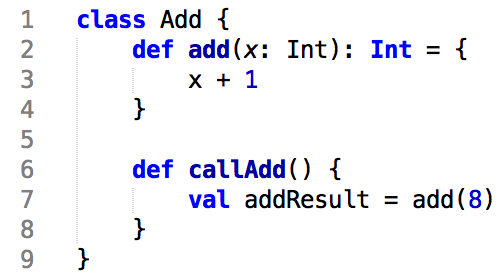
\includegraphics[scale=0.5]{figures/figure1}
\section{AST Approach} 

\subsection{Represent Data dependences with AST}
To represent data dependences, we can make use of information provided by Scala compiler. Since we use the compiler to change the program's behavior, it is very convenient to use informations from AST or ICode. ICode is a intermediate representation in Scala compiler between AST and byte code, which is translated into JVM byte code in the end. This section we focus on representing data dependences using information from ASTs. In section 4.1 we consider how to do it with ICode. 

Abstract Syntax Tree (AST) is a tree data structure used by compilers, which representing the parsed structure of a program. 
First let's see how the function definition \texttt{def add(...)\{...\}} is parsed into AST 
\\
\texttt{//Graph for the AST}
\\
Now we want to represent the dependences related to value \texttt{addResult}. 
First, notice see that \texttt{addResult} is an identifier, corresponding to \texttt{Ident} AST in Scala. And the function call \texttt{add(8)} is an \texttt{Apply} AST in Scala. Using \texttt{>>>} to represent dependence, then

\texttt{Apply >>> Ident}\\
which means the result of function call \texttt{add(8)} determines the value of \texttt{addResult}. However, the \texttt{Apply} and \texttt{Ident} should be given more specific names for analysis. For example, use \texttt{addResult} as the name of this \texttt{Ident} tree and \texttt{add} as the name of this \texttt{Apply} tree. Thus the information we provide to the analysis unit should be 

\texttt{add >>> addResult}\\
Similarly, other tree structures should have their specific names. For tree structures without a inherited suitable name, we will create a synthesis name, for example, a \texttt{Block} tree may use the name \texttt{Block124}, where \texttt{124} is the ID of this \texttt{Block} provided by the compiler. Here is the table about how names are given to various ASTs. 
\begin{table}[h]
\begin{tabular}{c|c}
\hline
AST & Name\\\hline
Apply(args, fun) &
Name of fun\\\hline
DefDef(mods, name, tparams, vparamss, tpt, rhs) &
name\\\hline
Block(stats, expr) & 
``Block" + AST ID\\\hline
Return(expr) &
``Return" + AST ID\\\hline
ValDef(mods, name, tpt, rhs) &
name\\\hline
If(cond, thenp, elsep) &
``If" + AST ID\\\hline
Select(qualifier, selector) & 
selector\\\hline
Match(selector, cases) &
``Match" + AST ID\\\hline
New(tpt) & 
``New" + AST ID\\\hline
Try(block, catches, finalizer) & 
``Try" + AST ID\\\hline
\end{tabular}
\end{table}
\\
In addition, we need another name for each function definition to represent its parameters. We use the function name appended by ``\$" to represent the parameters of this function. The usage of this special name will be clear in the following example. Here's the full example showing how the value of \texttt{addResult} is determined. The ``\texttt{>>>}" means ``determines". 

\texttt{8 >>> add\$}

\texttt{add\$ >>> x}

\texttt{x 1 >>> add}

\texttt{add >>> addResult}

The first two lines \texttt{8 >>> add\$} and \texttt{add\$ >>> x} say \texttt{8} is passed as the argument of function \texttt{add}. Here \texttt{add\$} acts as the bridge that connects \texttt{8} and \texttt{x}. Note that we don't use \texttt{8 >>> x} directly because number \texttt{8} is known when the function is called, while name of parameter \texttt{x} is only accessible inside the function definition. 

\subsection{Obtain Data Dependences at Runtime from AST} 
We've shown how to use information from AST to represent data dependences. Next problem is how can these information be passed to our analyzing module. 

The basic idea is, we can change the Scala program, using compiler plugins, to insert some ``log" operations inside the program as parts of the program itself. A ``log" operation is simply a function call to the analyzing module, taking the data dependence information as a string argument. So that when the program is executed, data dependence information is passed to the analyzing module simultaneously. 

Here is how we want to insert the ``log" operations into the program. 
\\
\\
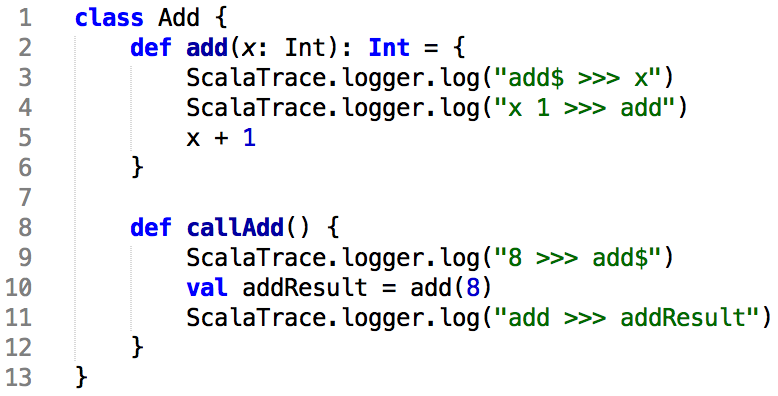
\includegraphics[scale=0.5]{figures/figure6}

Once the original program is modified into program above, data dependences \texttt{add\$ >>> x, x 1 >>> add, 8 >>> add\$, add >>> addResult} will be passed to analyzing module sequentially when it is executed. It is convenient to insert the ``log"'s after the program is parsed into AST. 

To explain how to insert the ``log"'s into ASTs, first we should know basically how Scala compiler works. Scala compiler has over 20 compilation phases. Almost all phases take an AST as input, modify the AST and pass it to the next phase. 

Our goal is to modify the AST by inserting our ``log" operations. Scala compiler plugin is a convenient tool to do this. A compiler plugin is a program written by user that acts as an additional compilation phase. The plugin can be inserted between almost any two standard compilation phases. Just like standard phases, a plugin also takes an AST as input, modify it and produce a new AST, which is passed to next phase. 

To insert ``log" operations, we should create ASTs for the function calls of \texttt{ScalaTrace.logger.log}, then insert them in the appropriate place of the original AST. Following shows a code snippet in our compiler plugin that creates such ASTs. 
\\
\\
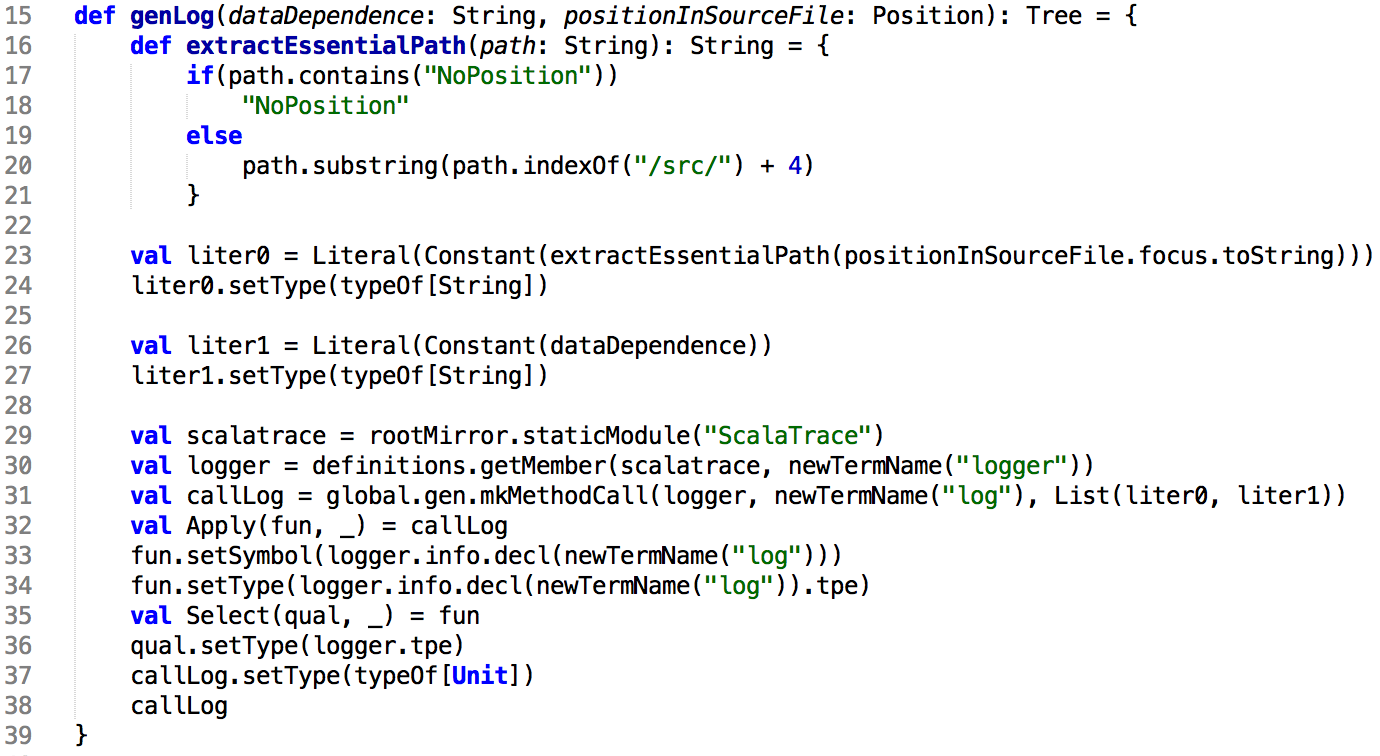
\includegraphics[scale=0.5]{figures/figure7}

Line 23 and 26 creates ASTs for two string arguments of \texttt{log} method. Line 31 creates the function call of \texttt{log}, which is an \texttt{Apply} AST. The compiler plugin should runs after standard phase \texttt{typer}. Because after \texttt{typer}, the names and types of ASTs are calculated, so that these can be used in the data dependence information.

However note that AST for \texttt{log} is created by us in the plugin, which runs after \texttt{typer}. So we have to set the types and symbols for it and its subtrees by ourselves so that it can be a legal tree for the following phases. That's why there are a lot of \texttt{setType}, \texttt{setSymbol} in the snippet above. 

Then our plugin traverses the original AST, calls genLog to create the ``log" ASTs and insert them at appropriate places. Following shows the ASTs before and after our plugin phase.
\\
\\
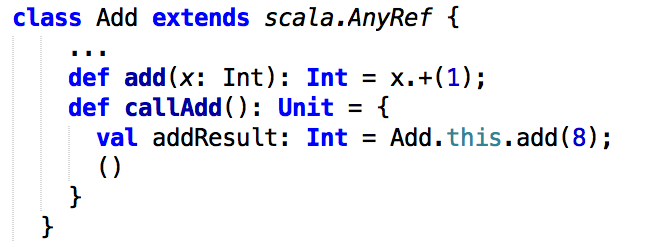
\includegraphics[scale=0.5]{figures/figure9}

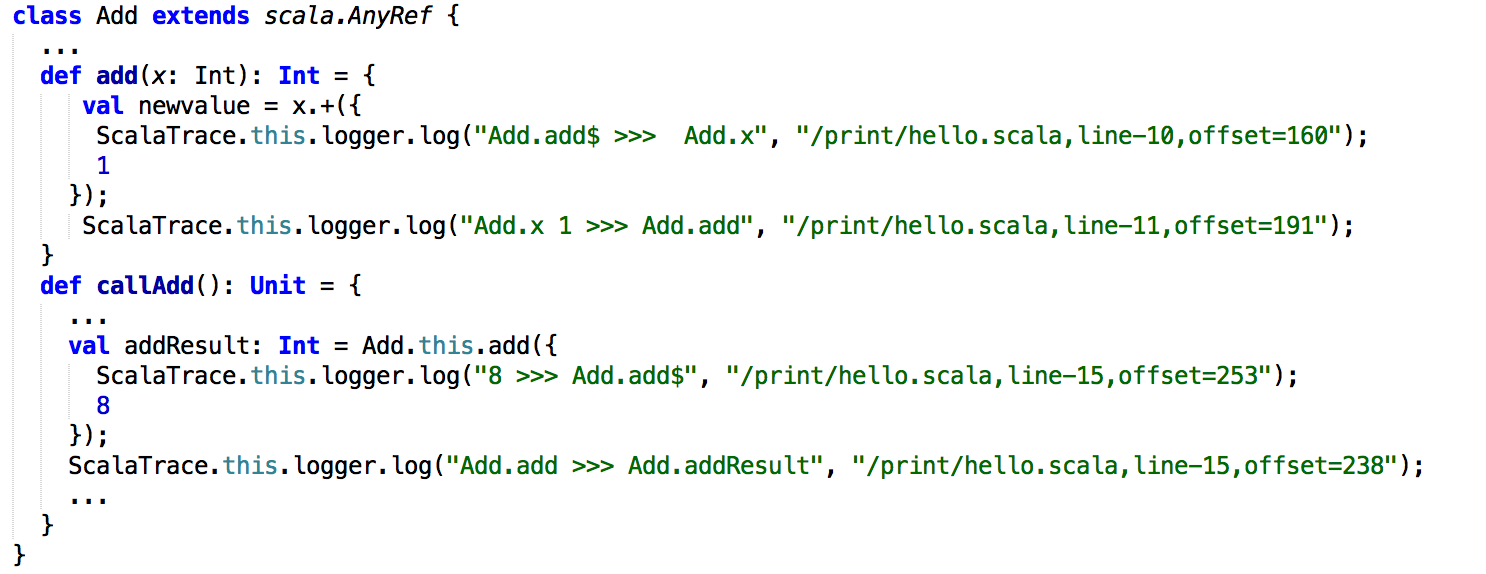
\includegraphics[scale=0.5]{figures/figure8} 
\subsection{Analyzing Data Dependences Extracted from AST}


\section{ICode Approach}
\subsection{Represent Data Dependences with ICodes}
ICode imitates push/pop operations of a stack machine. Each ICode instruction can first take some values as input from the stack, and then put its result onto the stack. Here's the table of main scala ICodes and their corresponding push/pop operations. 
\begin{table}[h]
\footnotesize
\begin{tabular}{c|p{5cm}|c}
\hline
ICode & Operations & Stack Operations \\\hline
THIS & loads ``this" on top of the stack & push 1\footnote{push 1 means pushing one value/object onto stack, similarly hereinafter.}\\\hline
CONSTANT & loads a constant on the stack & push 1\\\hline
LOAD\_ARRAY\_ITEM & loads an element of an array & pop 2, push 1\\\hline
LOAD\_LOCAL & load a local variable on the stack & push 1\\\hline
LOAD\_FIELD & load a field on the stack & pop 1, push 1\\\hline
LOAD\_MODULE & load a module on the stack & pop 1\\\hline
STORE\_ARRAY\_ITEM & store a value into an array at a specified index & pop 3\\\hline
STORE\_LOCAL & store a value into a local variable & pop 1\\\hline
STORE\_FIELD & store a value into a field & pop 2\\\hline
STORE\_THIS & store a value into the 'this' pointer & pop 1\\\hline
CALL\_PRIMITIVE & call a primitive function & pop n\footnote{n means the number of arguments, similarly hereinafter.}, push 1\\\hline
CALL\_METHOD & call a method & pop n, push 1\\\hline
NEW & create a new instance of a class & pop n, push 1\\\hline
CREATE\_ARRAY & create an array & pop n, push 1\\\hline
SWITCH & a switch instruction & pop 1\\\hline
CJUMP & jump according to the result of comparing two values & pop 2\\\hline
CZJUMP & jump according to the result of comparing with zero & pop 1\\\hline
THROW & throws an exception & pop 1\\\hline
DROP & drop one value from the stack & pop 1\\\hline
DUP & duplicate the top of the stack & pop 1, push 2\\\hline
LOAD\_EXCEPTION & load an exception & pop all, push 1\\\hline
\end{tabular}
\end{table}

With these operations on the stack, we can know exactly each value on the stack is produced and consumed by which instruction. Thus data dependences can be represented using a sequence of push/pop operations. Again we demonstrate with the running example to see how these push/pop operations are extracted from the ICode. 

First let's see how the simple \texttt{add} function is translated into ICode.
\\
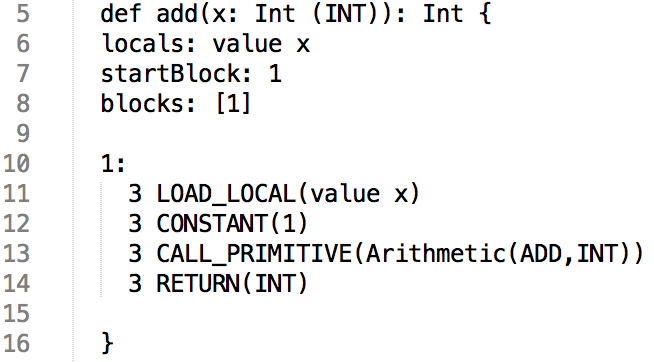
\includegraphics[scale=0.5]{figures/figure4}
\\
Our simple \texttt{add} function is translated into 4 ICodes. First, it loads the parameter \texttt{x} onto stack, then a constant \texttt{1}. After that, the \texttt{ADD} primitive operation is called. Finally, the function returns. The number \texttt{3} before these ICodes is the line number of corresponding source code. 

Here's the ICode for the assignment \texttt{val addResult = add(8)}\\
\\
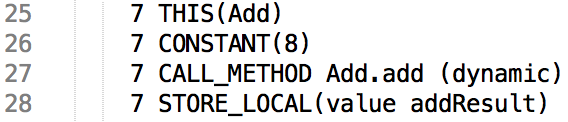
\includegraphics[scale=0.5]{figures/figure5}
\\
Again it can be represented by 4 lines of ICode. First it loads ``this" onto the stack, this is needed to call \texttt{add} method. Note that \texttt{add} is a method which consumes an object of \texttt{Add} class. Since here it is called inside the \texttt{Add} class, so ``this" object will be used. Then it loads the constant \texttt{8}, as the argument for \texttt{add} method. The third ICode calls \texttt{add} method. After this ICode, the ICodes of \texttt{add} method will be executed. When the \texttt{add} call finishes, store its result into \texttt{addResult}. 

Putting it all together, here's the sequence of ICodes being called when the assignment \texttt{val a = add(8)} is executed, with push/pop operations for each ICode shown on the right.
\begin{table}[h]
\footnotesize
\begin{tabular}{c|c|c}
\hline
Step & ICode & Operation\\\hline
\texttt{1} & \texttt{THIS(ADD)} & \texttt{push @this}\\\hline
\texttt{2} & \texttt{CONSTANT(8)} & \texttt{push 8}\\\hline
\texttt{3} & \texttt{CALL\_METHOD Add.add (dynamic)} & \texttt{pop x, pop @this}\\\hline
\texttt{4} & \texttt{LOAD\_LOCAL(value x)} & \texttt{push x}\\\hline
\texttt{5} & \texttt{CONSTANT(1)} & \texttt{push 1}\\\hline
\multirow{4}{*}{\texttt{6}} & \multirow{4}{*}{\texttt{CALL\_PRIMITIVE(Arithmetic(ADD, INT))}} & \texttt{pop @operand1} \\
& & \texttt{pop @operand2} \\
& & \texttt{@operand1 @operand2 >>> @result} \\
& & \texttt{push @result}\\\hline
\texttt{7} & \texttt{RETURN} & \\\hline
\texttt{8} & \texttt{CALL\_METHOD Add.add (dynamic)} & \texttt{push @result}\\\hline
\texttt{9} & \texttt{STORE\_LOCAL(value addResult)} & \texttt{pop addResult}\\\hline 
\end{tabular}
\end{table}

In our push/pop operations above, \texttt{push <something>} means putting \texttt{<some-\\thing>} on the stack. \texttt{pop <something>} means storing the top of stack into \texttt{<something>} then pop the stack. Sometimes we need \texttt{>>>} to represent data dependences directly. For example \texttt{a b >>> c} means the value of \texttt{c} is determined by \texttt{a} and \texttt{b}. 


\subsection{Obtain Data Dependences at Runtime from ICodes}
Now we know how push/pop operations that exactly describes data dependences can be extracted from ICodes. In this section let's focus on how to insert ``log" function calls into ICodes. 

We modify the icode phase of scala compiler 2.11 to insert additional ICodes for each original ICode. These additional ICodes calls the ``log" function, passing push/pop operations to the analyzing unit. 

Following shows the ICodes to call ``log" function. 
\\

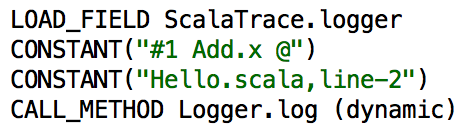
\includegraphics[scale=0.5]{figures/figure11}

Our ``log" function is a method of Logger class. The program and our analyzing tool will interfere through \texttt{ScalaTrace} module, which is a final java class. \texttt{logger} is a static field of \texttt{ScalaTrace}. 

To call \texttt{ScalaTrace.logger.log}, \texttt{ScalaTrace.logger} should be loaded first. This is done by the first \texttt{LOAD\_FIELD} ICode. Then two String arguments, line number and push/pop operation, needed by \texttt{log} should be put on stack. We can do this using two \texttt{CONSTANT} ICodes. Finally, \texttt{CALL\_METHOD} ICode calls \texttt{Logger.log}, using \texttt{ScalaTrace.logger} as the object to call this method, with the two String constants as arguments. 

For each ICode generated from the original program, these additional ICodes will be added before them, to passing the position and push/pop operations of original ICodes to our analyzing module. Following figure shows ICodes of our \texttt{add} function, with additional ICodes. 

\subsection{Analyze Data Dependences Extracted from ICodes}   
From section 4.2 we know how push/pop operations and code positions are passed to our analyzing module. This section focus on how to analyze these information are used to analyze data dependences, and find out dead codes. 

\subsubsection{Build Data Dependence Graph}
Here's the basic idea of our analyzing algorithm. 
Our analyzing modules maintains a stack to imitate every push/pop operation of the program's original ICodes. In this way, whenever an ICode pop something from the stack as an operator, our analyzing module knows exactly which object it gets. 
For example, at some time, an object \texttt{ObjA} is push on the stack in source code position \texttt{file1,line-21}. Later on, \texttt{ObjA} is popped from the stack in source code position \texttt{file2,line-34}. This means \texttt{file2,line-34} has a data dependence on \texttt{file1,line-21}. 

In this way, the data dependences between all lines of source codes in the original programs can be detected. Thus we can build a dependence graph in memory to maintain such relationships. Vertices in the graph corresponds to lines in the source code. Vertices are connected by directed edges. If there's an edge from Vertex A to Vertex B, that means source code line of Vertex B depends on that of Vertex A. 
\\
\\
\texttt{TODO Sample Dependence Graph}
\subsubsection{Search for Dead Codes}
To search for dead codes within the dependence graph, a target must first be assigned. A target is an variable name in the program that the user considers as the final result of the program. For example, suppose the program is our Scala compiler, then the target can be \texttt{jclassBytes}, the variable storing the final java byte code, which is the final product of Scala compiler. 

The target should be assigned before the program is executed. Then after the program lanches, our analyzing module will build the dependence graph gradually. Then, when the program is writing the target variable, a push operation \texttt{push <target>} will be passed to the analyzing module, along with its source code line. Then vertex corresponding to this source code line will be marked as useful, as well as all descendants of this vertex. 
\subsubsection{Get the Result}
The last question is how to obtain the useless source code lines. Since we only mark source code lines as useful or useless, a straight forward idea is we can simply dump all the source code lines and all  the useful source code lines into two separate files when the compilation finishes, then take the difference of these two files to get the useless lines. 

However, to do this the program must be able to inform the analyzing module before it terminates so that the analyzing module can dump the result to files. As the program terminates, all the result in our analyzing module will disappear. This requires special treatment to inserting function calls other than ``log" to code segments that the program will execute before terminating. It is extremely hard to identify such code segments at compile time. 

Thus whenever a new source code line is executed or being marked as useful, the analyzing module has to write it to the file. Because all the actions of our analyzing module is activated function calls from the program, and it doesn't know when the program will terminate, it has to write the result incrementally. 

\section{Experiments and Results} 
\end{document}